\chapter{子板 HDMI 回显工程}

\section{职责与数据通路}

显示子板(MLKPAI-F01,EG4D20EG176)是纯接收显示设备:从主板 ETHB 镜像口接收
千兆视频码流,还原为 1280$\times$720 图像后以 HDMI 720p60 实时输出。板上无命令
通路、零参数调节;协议栈发送侧请求恒为零(纯二层接收,ping 不通属正常)。数据
通路按三个时钟域组织(图~\ref{fig:subboard}):\textbf{clk\_125} 域完成 RGMII
接收(PLL2 控制采样相位 + IDDR)、rgmii\_cdc 跨域、MAC/IP/UDP 协议栈解析与帧
重组;\textbf{fdma\_clk 150M} 域完成 uidbuf 三缓冲与 FDMA 对合封 DDR1(16MB)的
读写;\textbf{pclkx1 75M} 域完成 720p60 视频时序、OSD 叠加与 TMDS 编码输出。

\begin{figure}[H]\centering
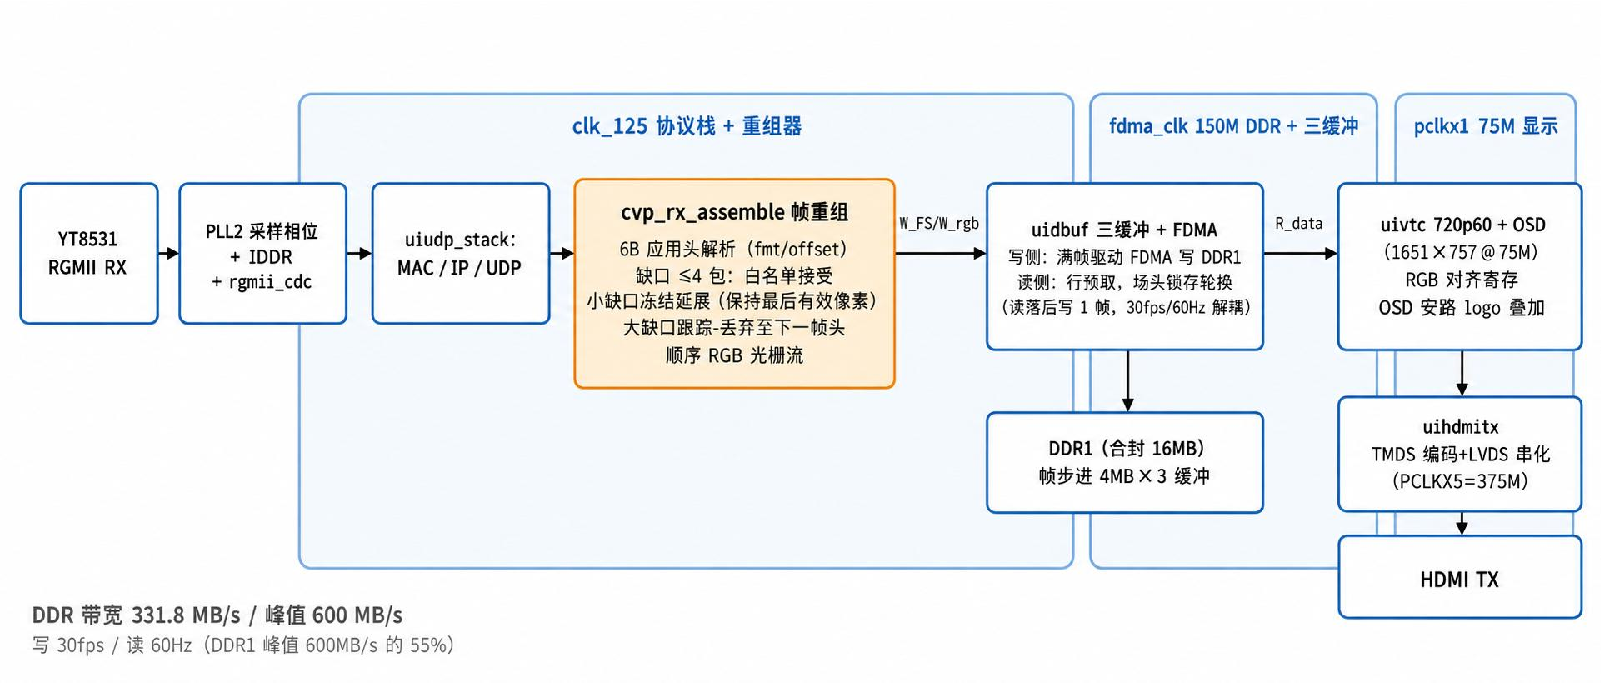
\includegraphics[width=\textwidth]{figs/fig_subboard.pdf}
\caption{子板数据通路:三个时钟域与帧重组/三缓冲/显示输出}
\label{fig:subboard}
\end{figure}

协议栈沿用厂商 UDP 例程(27 文件),其中 MAC 接收层有一处有意修改:广播分支由
"仅 ARP 放行"改为"ARP 或 IP 均放行"(视频流目的 MAC 为广播),IP 层仍有目的
地址精确过滤兜底。本地 IP 设为视频流的目的地址(192.168.1.100),端口 6000 收
视频、6002 状态包按格式字节丢弃。

\section{帧重组器 cvp\_rx\_assemble}

帧重组器是子板的核心自研模块,解决的问题:协议栈输出"无反压、按包到达顺序"的
UDP 载荷字节流,而三缓冲写侧需要"每帧恰好 921{,}600 像素、帧同步脉冲分隔"的
顺序视频流——两者之间隔着丢包、乱序容忍与速率整形三道鸿沟。算法为 PC 收图脚本的
硬件化,适配无反压约束:

\begin{enumerate}[nosep]
\item \textbf{输入侧}(每输入字节 1 拍):解析 6 字节应用头,判定接受条件为
"格式 = 视频 且 偏移 + 1440 $\leq$ 帧长 且(偏移 = 0 新帧标记,或偏移 $\geq$
已承诺位置 且 缺口 $\in\{0,1,2,3,4\}\times$1440B 白名单)"。白名单归纳保证接受
的包恒为整包对齐。接受的包:载荷压入 4096B staging FIFO,描述符(目标偏移)入
8 深队列;偏移为 0 的包先额外插入一条帧尾描述符。
\item \textbf{输出侧}(描述符状态机,严格顺序):S\_FILL 从已输出位置到本描述符
偏移,用最后一个有效 RGB 像素冻结延展,完成缺口对齐;S\_DATA 从 staging 弹 3 字节拼
RGB 输出 480 像素;S\_FS(帧尾描述符)也用最后有效像素延展到帧尾,再发帧同步并清零
位置。
\item \textbf{不变量}:任意两个帧同步脉冲之间恰好输出 921{,}600 像素(实像素 +
冻结延展像素)——保证写侧 FDMA 每帧固定突发数、永不因短帧卡死。
\item \textbf{丢包行为}:连续缺失 $\leq$4 包时接受后续包,缺口以最后有效像素冻结
延展;缺口 $>$4 包时跟踪并丢弃当前帧剩余数据,直到下一帧偏移 0 自动重新同步,
上一帧余量仍由最后有效像素延展;码流彻底中断则最后一完整帧静止显示。
\item \textbf{跟踪-丢弃}:帧尾/洞填充期间(最长约 74 万拍)staging 无法排空,被
水位挡住但通过格式/界内/顺序检查的包\textbf{推进已承诺位置、不入队},避免
committed 停滞引发缺口级联;填充结束即重新同步,损失只限丢包当帧。
\item \textbf{staging 水位论证}:冻结延展期输出 1 像素/拍,对输入 1B/拍,峰值约
2 包(2.9KB)< 4096B;数据期弹 3B/拍 $\geq$ 入速,迅速回落。
\end{enumerate}

\section{DDR 三缓冲与显示输出}

写侧 30\,fps 与读侧 60\,Hz 异步解耦由三缓冲完成:uidbuf 以"写满整帧驱动 FDMA
写、读侧行预取 FDMA 读"的方式访问合封 DDR1(16MB,帧步进 4MB $\times$ 3 缓冲),
场头锁存切换缓冲、读落后写一帧。带宽核算:写 110.6 + 读 221.2 = 331.8\,MB/s,
占 DDR1 峰值 600\,MB/s 的 55\%,余量充足;若需进一步降带宽,后备开关为 RGB565
(数据宽度参数化)。显示侧 uivtc 产生 720p60 时序(1651$\times$757@75M),读出
RGB 与数据使能同拍打一拍寄存后送 uihdmitx(TMDS 编码 + LVDS 串化,
PCLKX5 = 375M);右上角叠加安路 logo OSD(16384$\times$9 位图 + 125 色调色板,
readmemh 初始化)。

\section{时钟与资源}

全板 6 个时钟域:clk\_125(协议栈+重组器)、gmii\_rxc/PLL2(PHY 接收,rgmii\_cdc
跨出)、fdma\_clk 150M(DDR+三缓冲)、pclkx1 75M(显示)、pclkx5 375M(串化
原语内部)、clk\_12\_5(PHY 复位时序);4 个 PLL 全部占用(器件上限 4),时钟组
在 SDC 中显式声明。RGMII 采样相位由 PLL2 CPHASE 控制——采样相位随电源状态漂移
是偶发丢包的根源,诊断 LED 直接指示 CRC 状态,配合 CPHASE 盲扫脚本可求稳定采样
点。资源占用:LUT 7556/19600(38.9\%)、BRAM 44/64。

\section{验证体系}

子板建立三层仿真回归(\verb|tools/sim/|,Python 生成含正确 CRC 的 RGMII 线上
向量注入,期望光栅逐字节比对):\textbf{协议/重组场景回归}(8 场景:完整/丢 1 包/
整帧丢/重复/乱序/坏 FCS/缺 6 包/心跳,8/8 通过);\textbf{全分辨率真机工况回归}
(1920 包/帧 $\times$ 11 帧逐字节比对);\textbf{专项压力测试}(DDR 仲裁 + 刷新
压力扫描、OSD 落点账本逐像素 diff = 0,含 2\,ms 总线黑窗注入的仲裁鲁棒性验证)。
上板验收:HDMI 显示正常、logo 正常;偶发丢包造成的瞬时冻结带由缺口冻结延展缓解
(旧版实现曾以黑色填充,当前版本改为保持最后有效像素)。
